%摘要
\section*{Data Ingestion Tools}
使用华为云ECS服务器,实现本次作业中的任务一和任务四

%介绍
\section{任务一:使用 Apache Kafka 进行数据流}

\subsection{下载最新版本的kafka并使用scp命令上传到云服务器}
\begin{figure}[H]
  \centering
  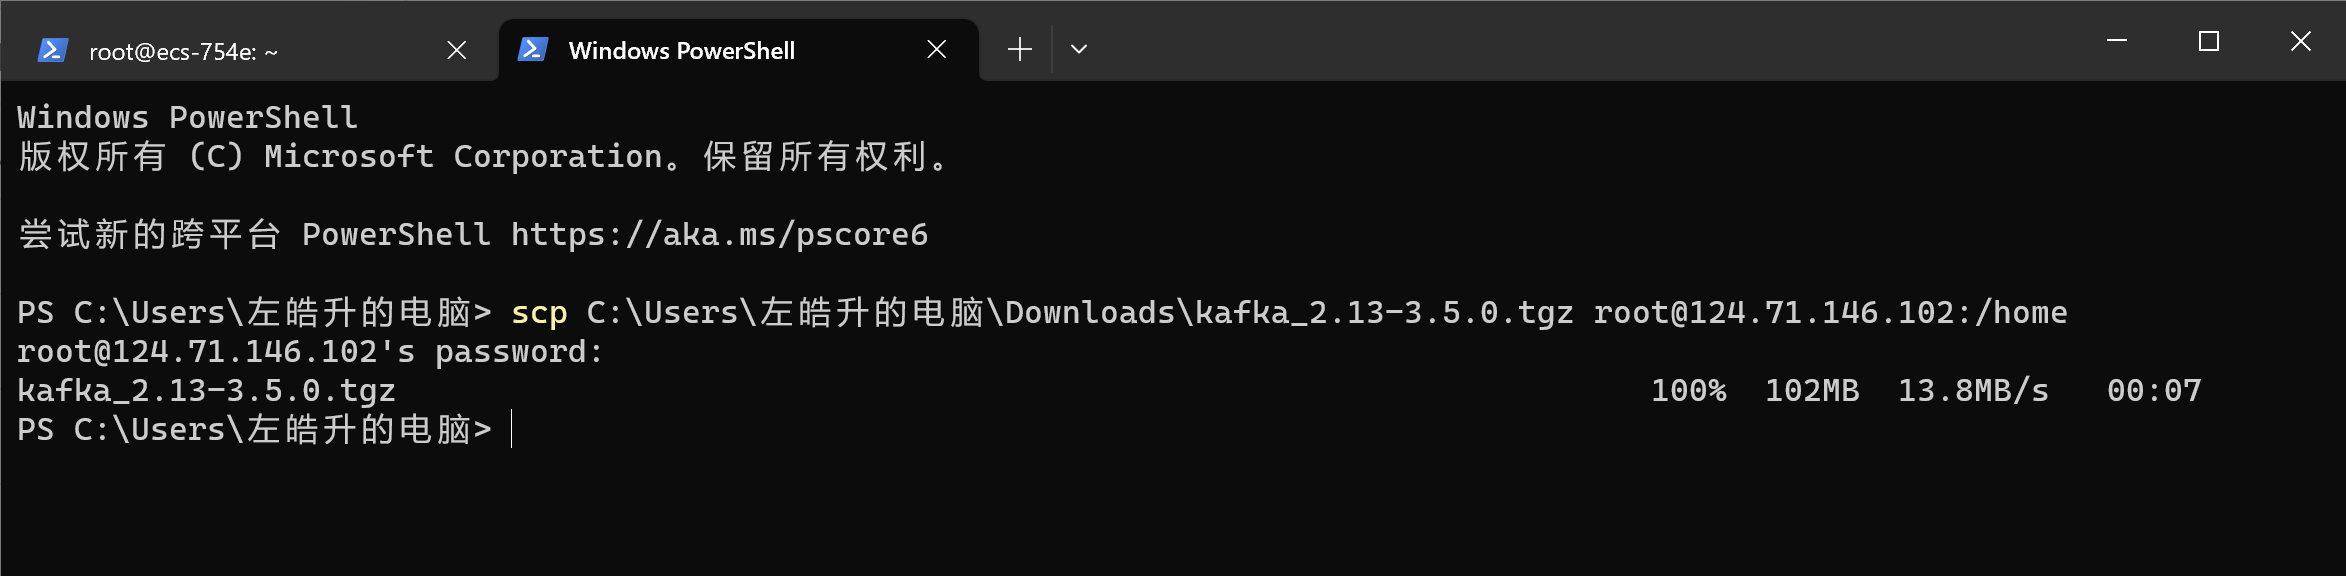
\includegraphics[width=\textwidth]{figure/1.png}
  \caption{下载上传}
  \label{fig:my_label}
\end{figure}

\subsection{SSH连接服务器,解压上传的tgz并进入解压后的文件夹}
\begin{figure}[H]
  \centering
  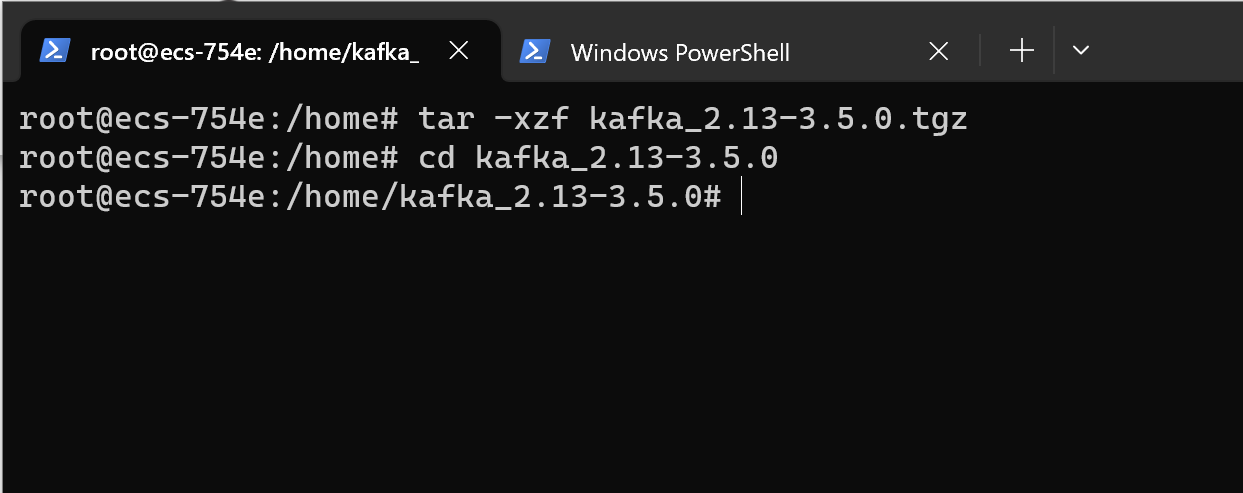
\includegraphics[width=\textwidth]{figure/2.png}
  \caption{解压}
  \label{fig:my_label}
\end{figure}

\subsection{启动zookeeper}
bin/zookeeper-server-start.sh config/zookeeper.properties
\begin{figure}[H]
  \centering
  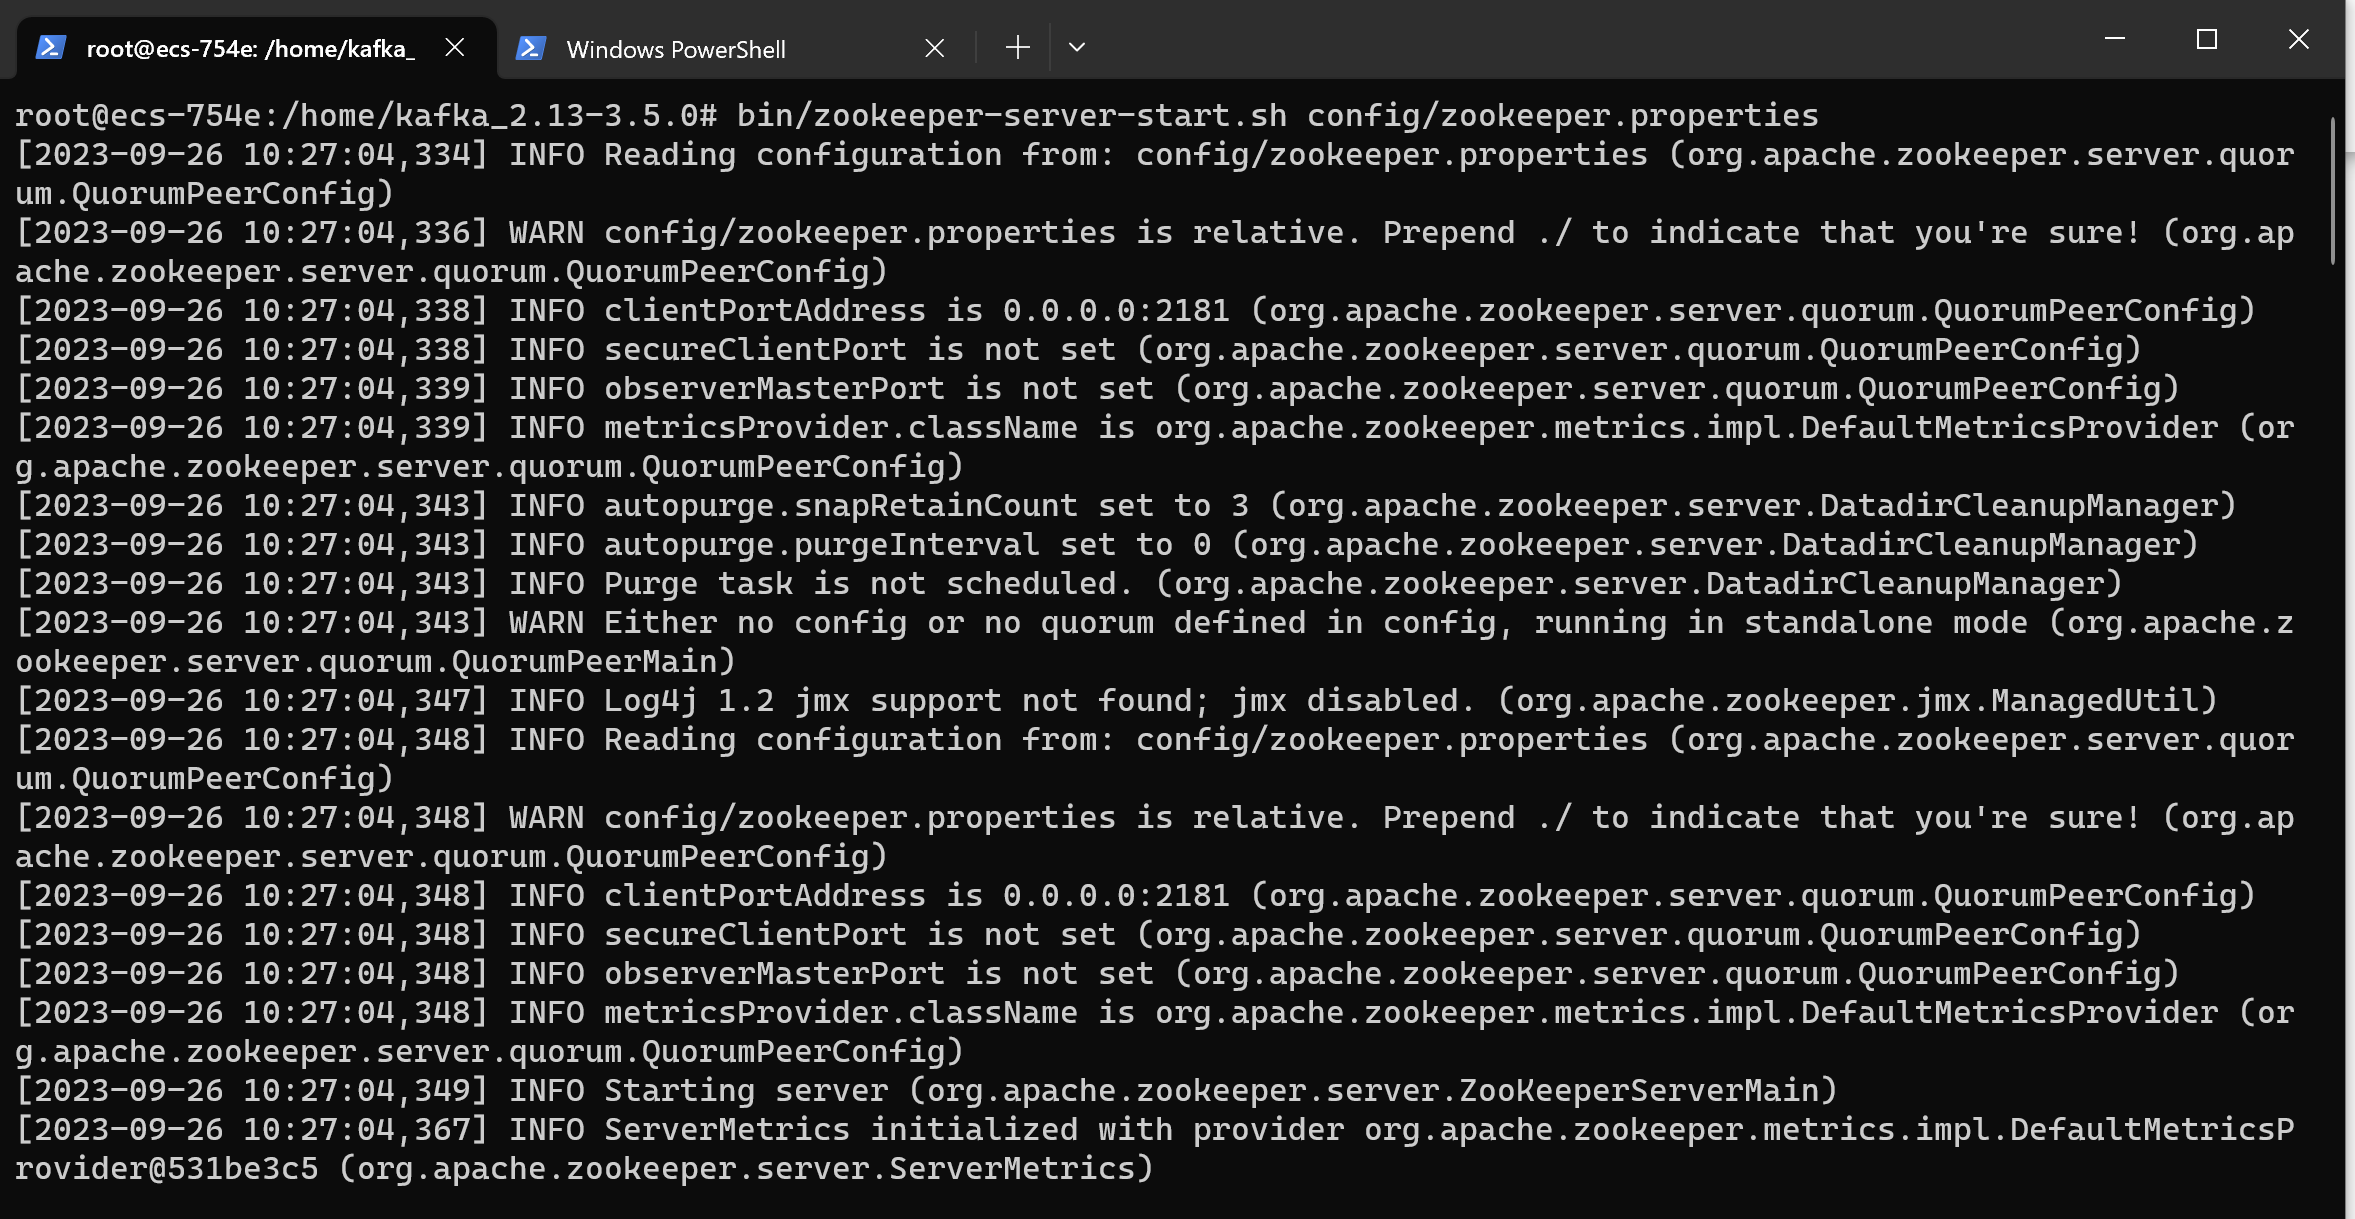
\includegraphics[width=\textwidth]{figure/4.png}
  \caption{运行1}
  \label{fig:my_label}
\end{figure}
\begin{figure}[H]
  \centering
  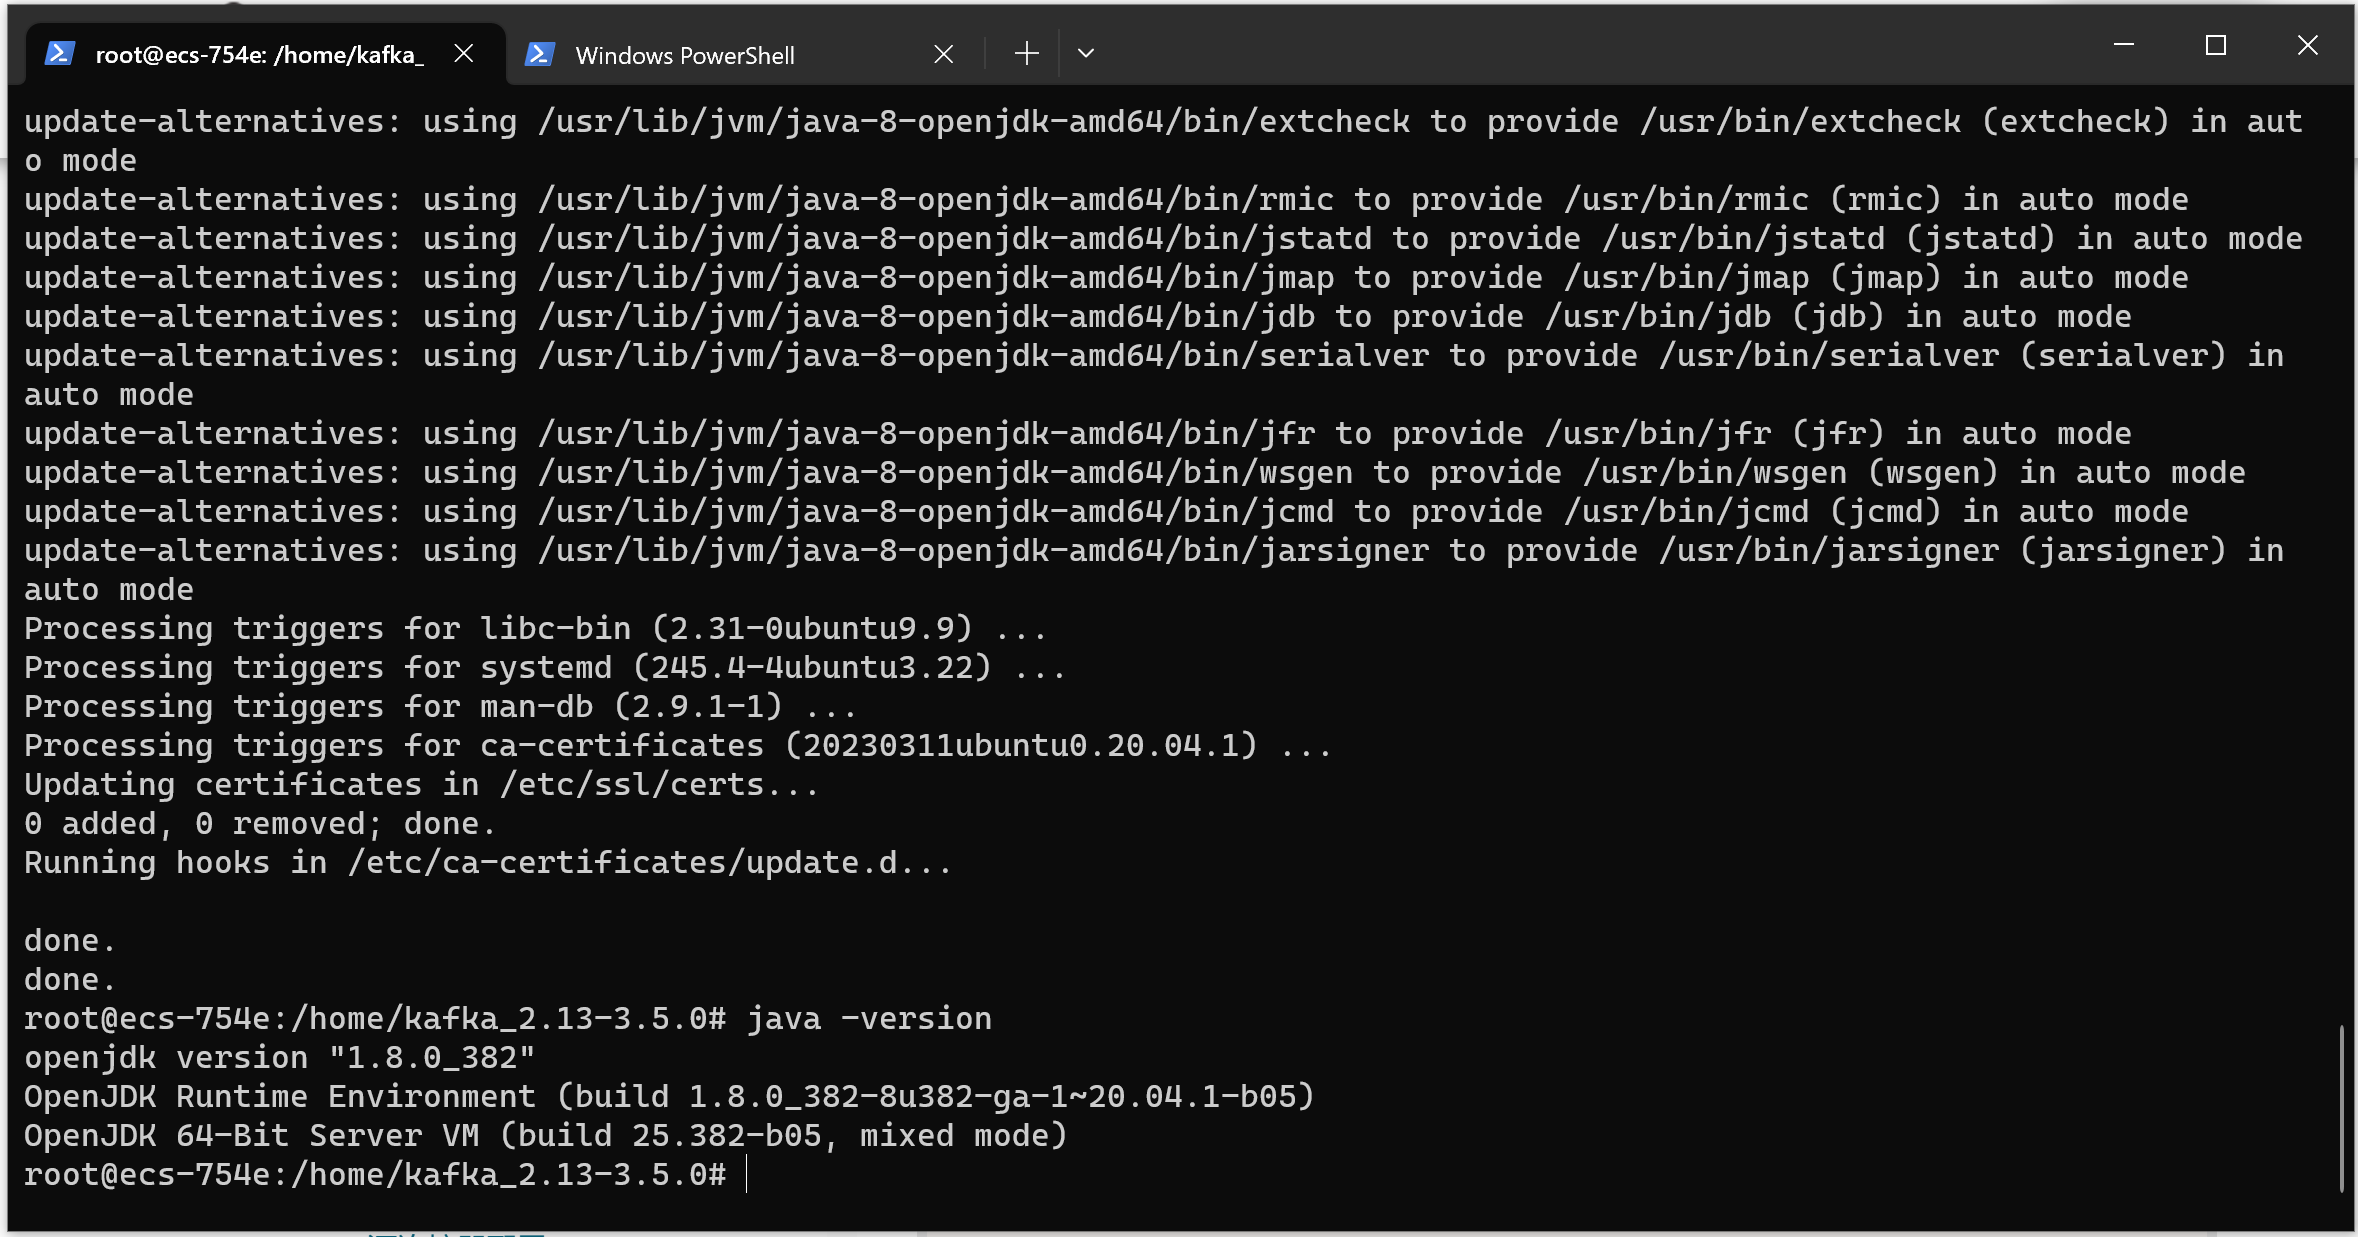
\includegraphics[width=\textwidth]{figure/3.png}
  \caption{运行2}
  \label{fig:my_label}
\end{figure}

\subsection{启动server}
bin/kafka-server-start.sh config/server.properties
\begin{figure}[H]
  \centering
  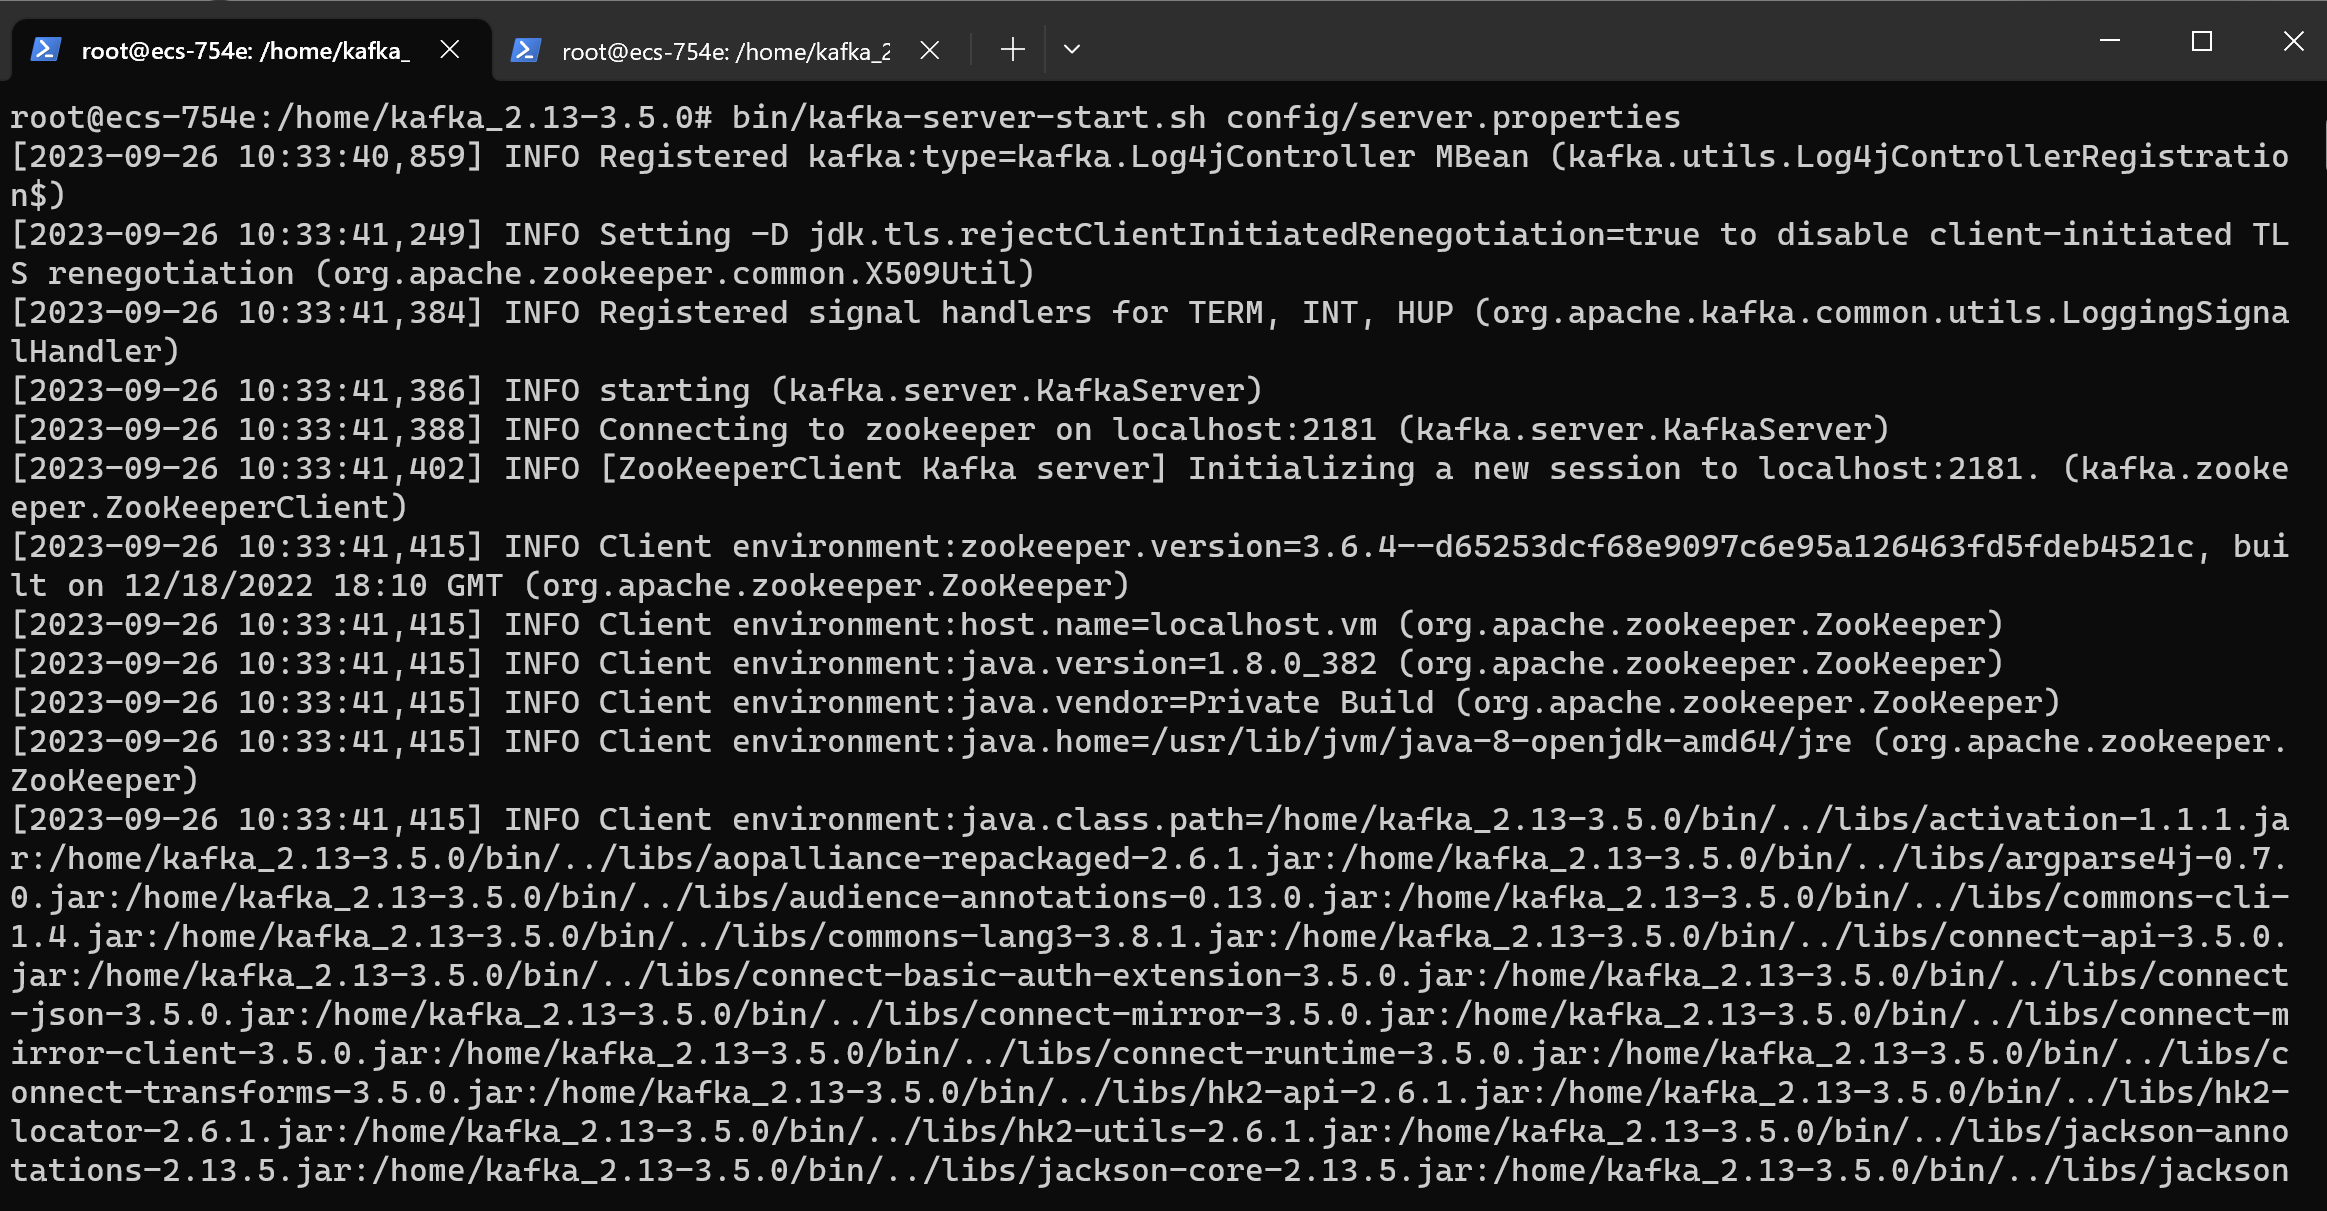
\includegraphics[width=\textwidth]{figure/5.png}
  \caption{运行3}
  \label{fig:my_label}
\end{figure}

\subsection{创建一个主题}
打开一个新终端\\
bin/kafka-topics.sh --create --topic quickstart-events --bootstrap-server localhost:9092
\begin{figure}[H]
  \centering
  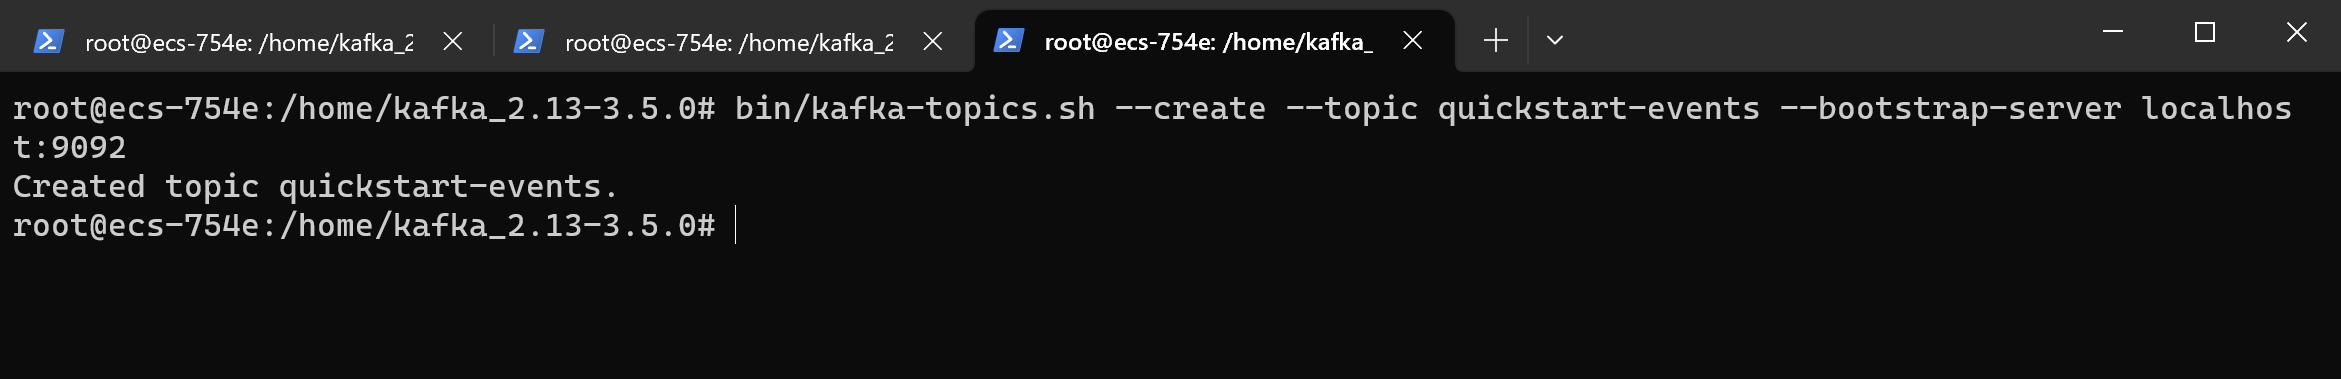
\includegraphics[width=\textwidth]{figure/6.png}
  \caption{创建主题}
  \label{fig:my_label}
\end{figure}

\subsection{打开生产者,将事件写入主题}
bin/kafka-console-producer.sh --topic quickstart-events --bootstrap-server localhost:9092
\begin{figure}[H]
  \centering
  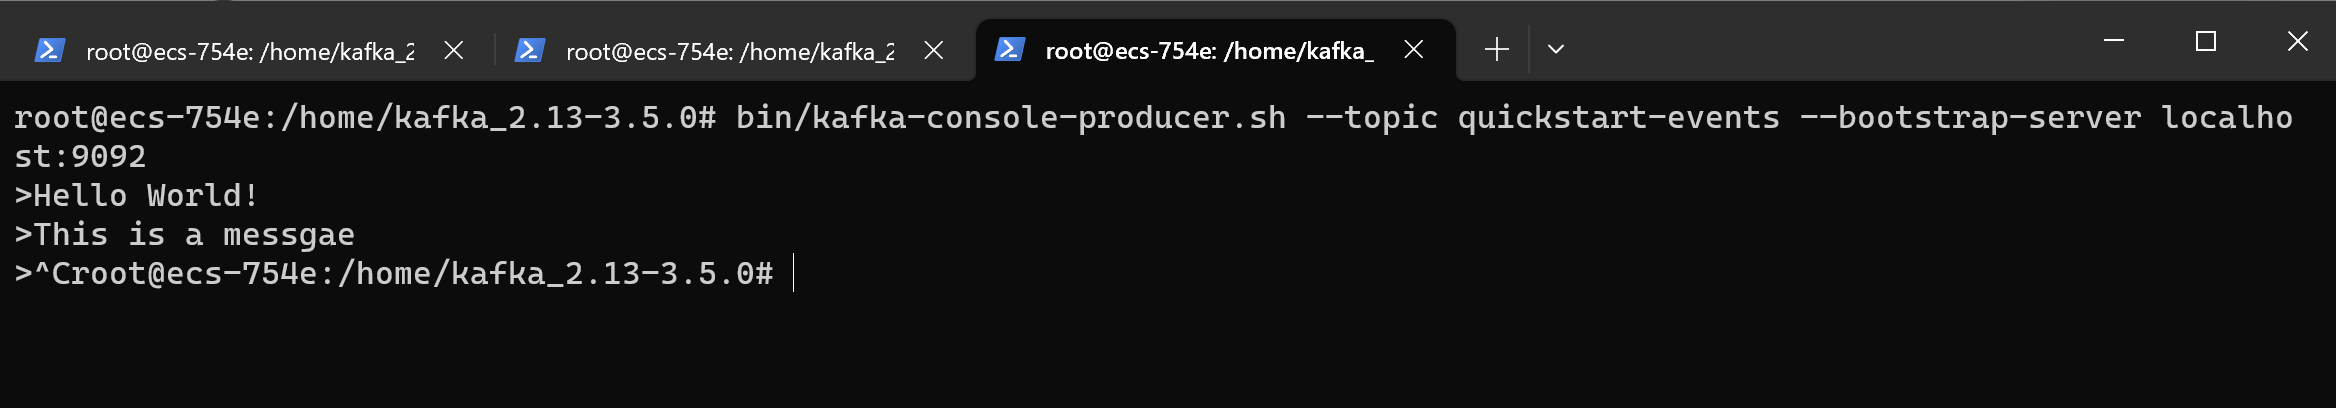
\includegraphics[width=\textwidth]{figure/7.png}
  \caption{创建主题}
  \label{fig:my_label}
\end{figure}

\subsection{打开消费者,读取事件}
bin/kafka-console-consumer.sh --topic quickstart-events --from-beginning --bootstrap-server localhost:9092\\
成功读取到了生产者的信息
\begin{figure}[H]
  \centering
  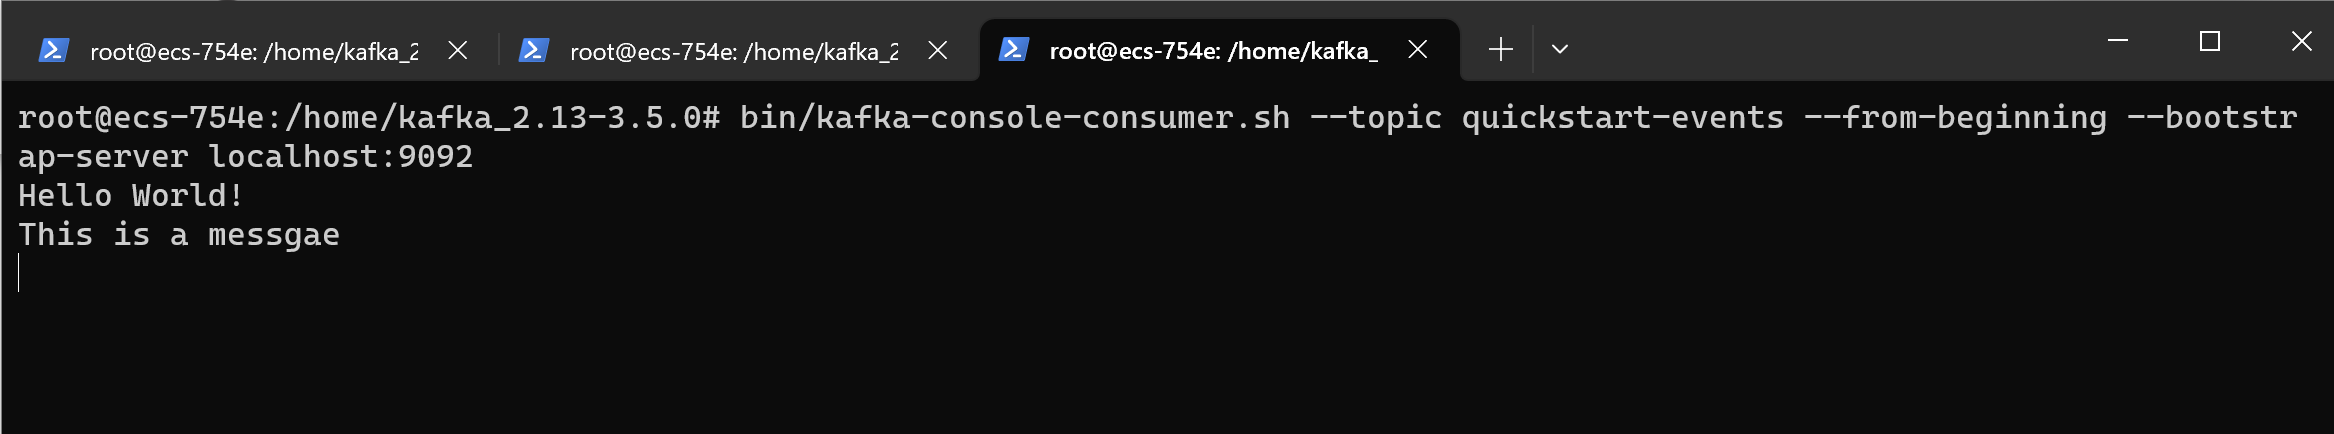
\includegraphics[width=\textwidth]{figure/8.png}
  \caption{阅读事件}
  \label{fig:my_label}
\end{figure}
确认了kafka主题中的信息,实验成功

\section{任务四:使用 Flume 收集日志}
\subsection{安装hadoop环境}
在上一次作业的某次尝试中,已经在我的ECS中安装好了java环境和hadoop,没有留下截图。参考了阿里云手册,过程较为简单\\


\subsection{将本地下载的Flume上传到云服务器}
\begin{figure}[H]
  \centering
  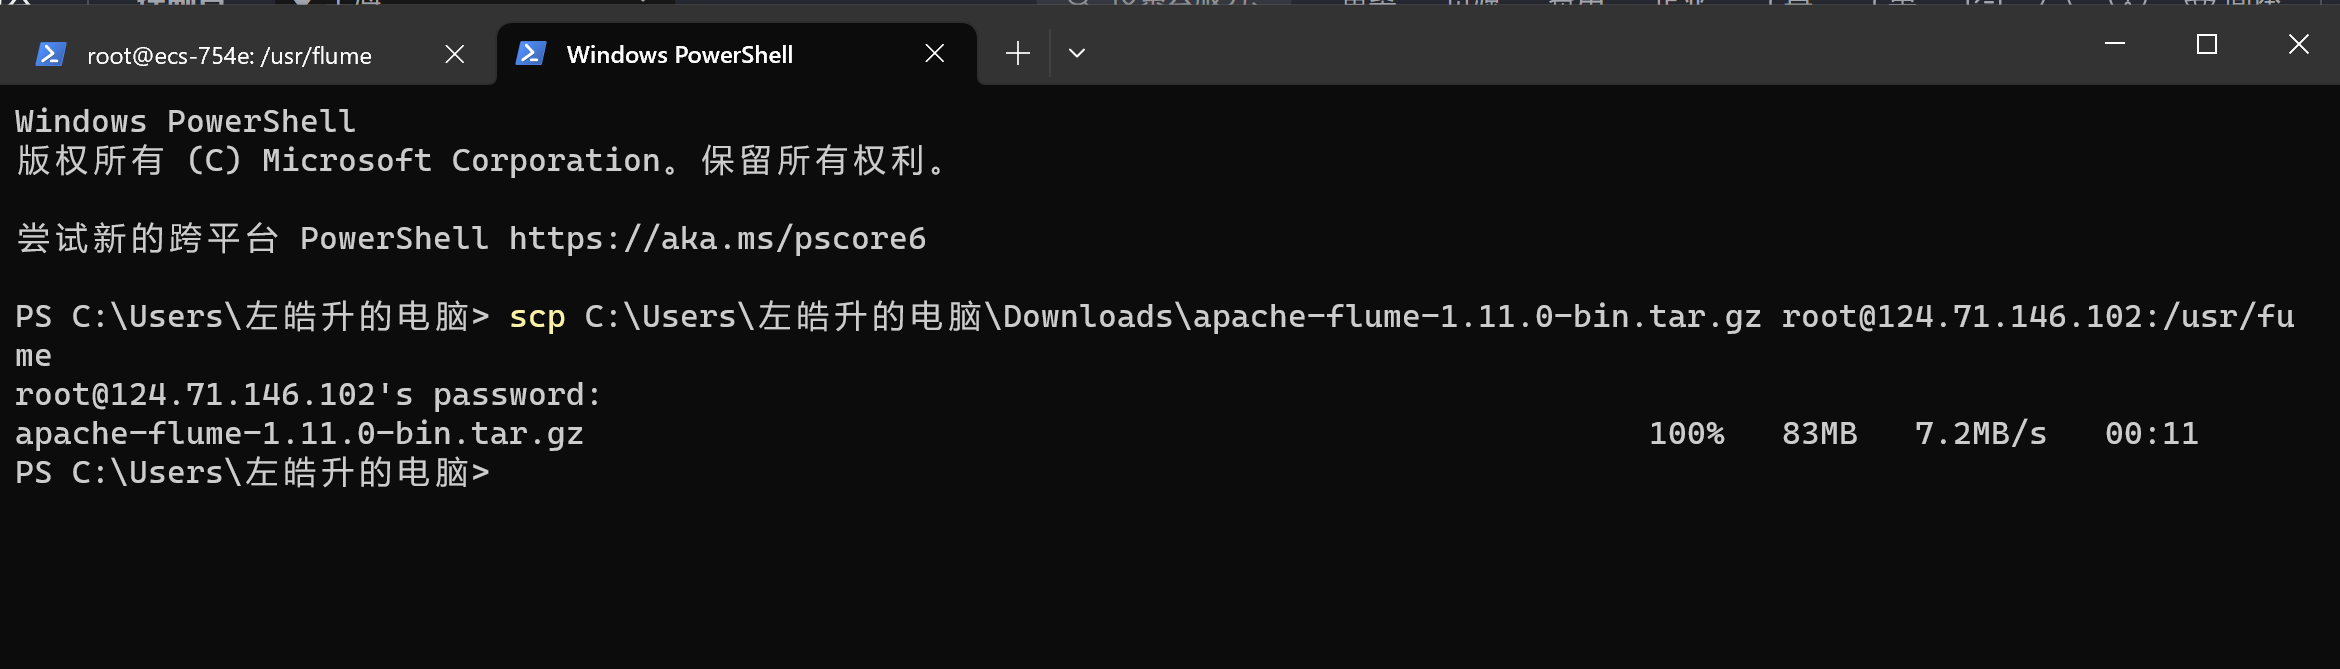
\includegraphics[width=\textwidth]{figure/11.png}
  \caption{上传}
  \label{fig:my_label}
\end{figure}

\subsection{SSH连接服务器解压并进入conf文件夹}
\begin{figure}[H]
  \centering
  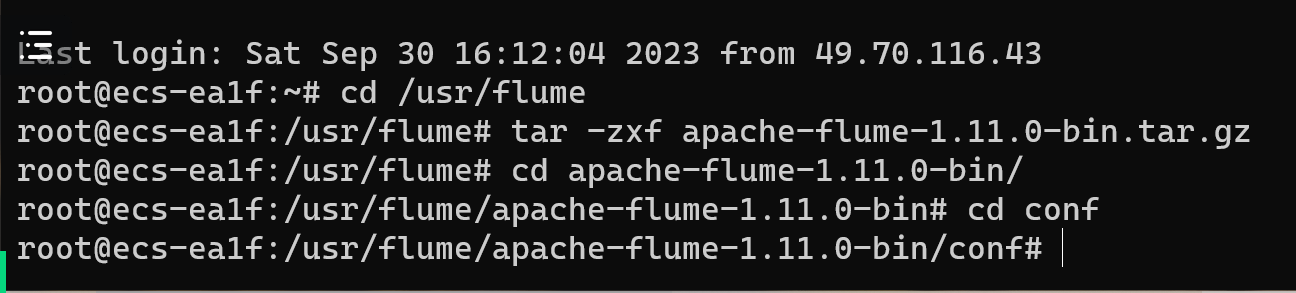
\includegraphics[width=\textwidth]{figure/12.png}
  \caption{解压}
  \label{fig:my_label}
\end{figure}

\subsection{新建.conf文件并写入配置文件}
\begin{figure}[H]
  \centering
  
\includegraphics[width=\textwidth]{figure/新建.conf.png}
  \caption{新建.conf}
  \label{fig:my_label}
\end{figure}
\begin{figure}[H]
  \centering
  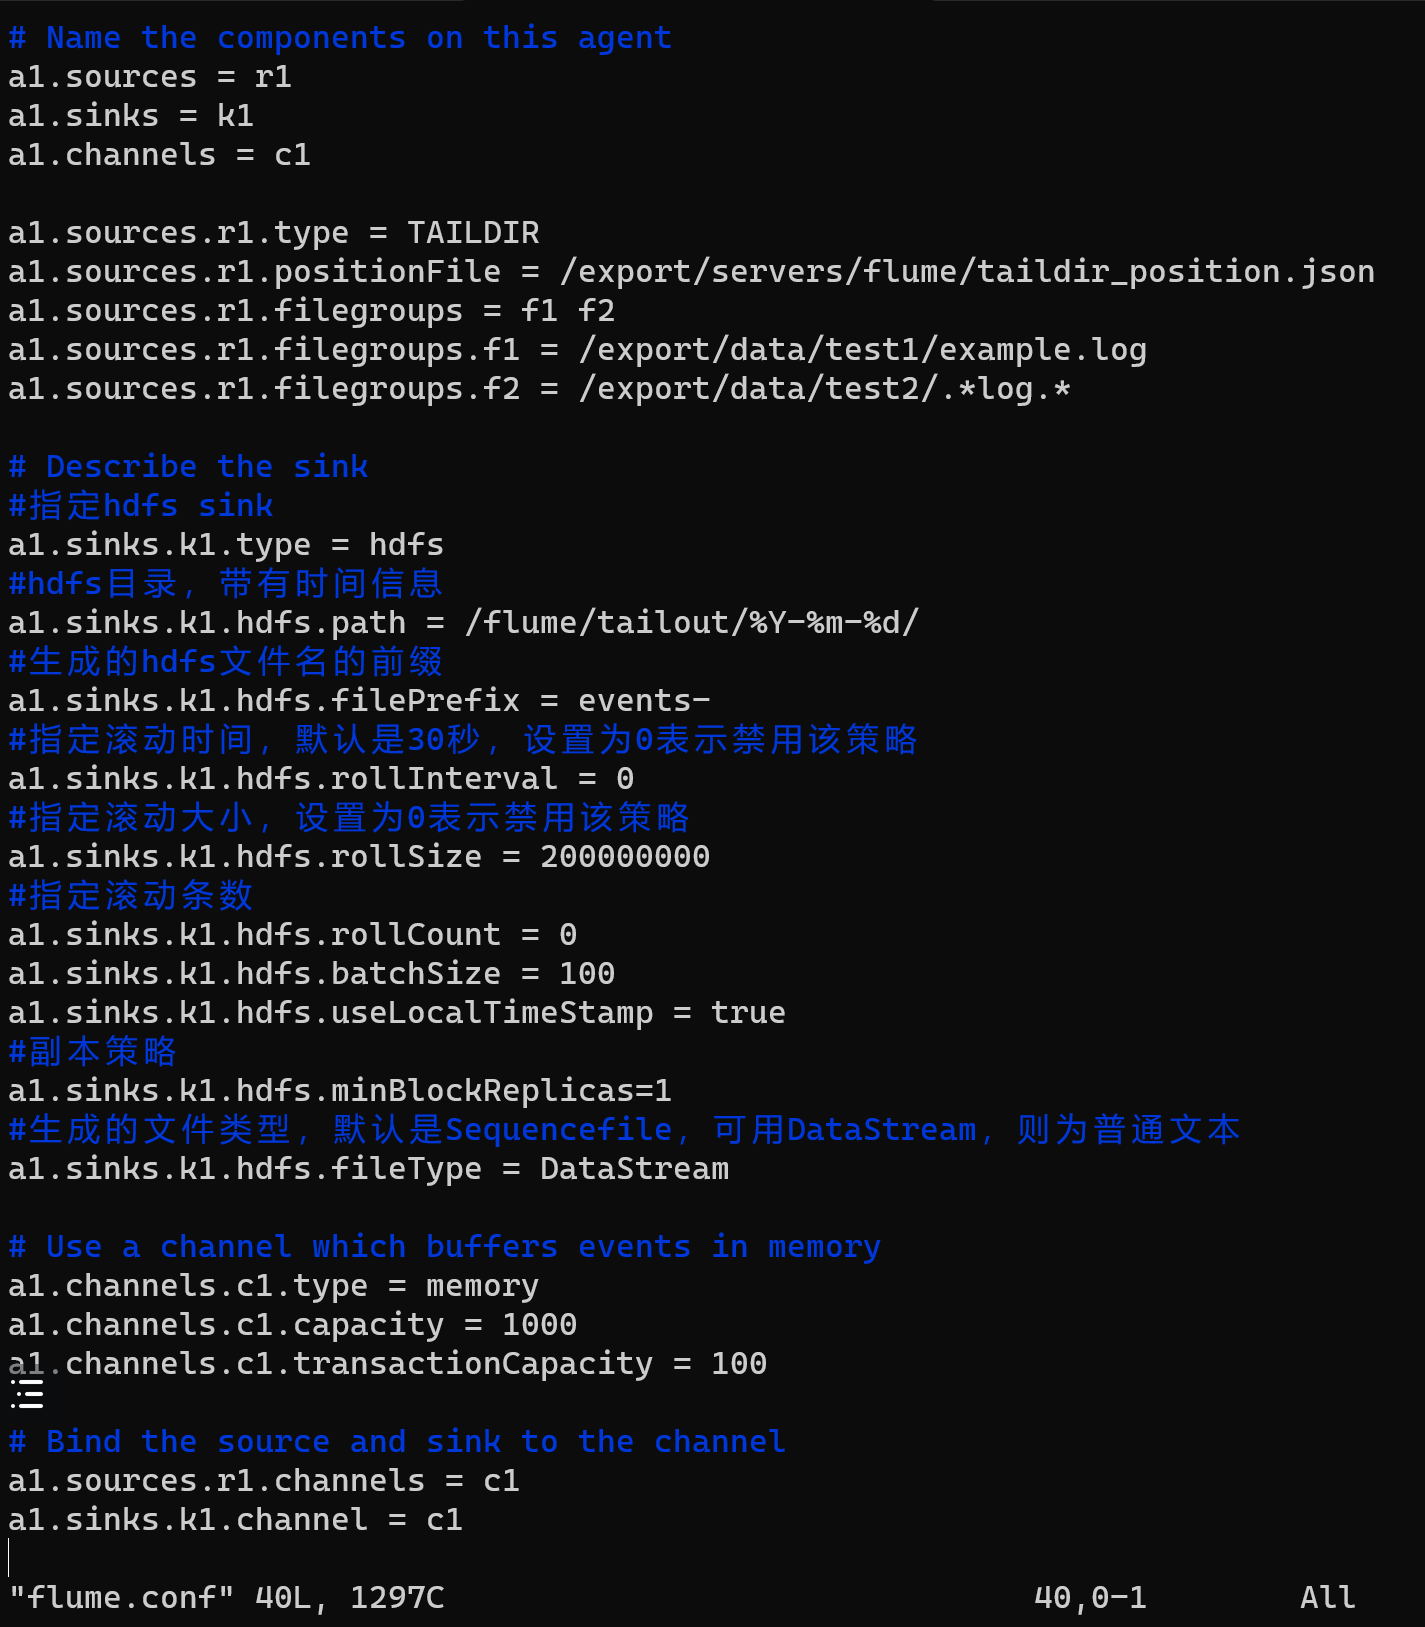
\includegraphics[width=\textwidth]{figure/配置文件.png}
  \caption{上传}
  \label{fig:my_label}
\end{figure}

\subsection{新建文件夹和.log文件}
\begin{figure}[H]
  \centering
  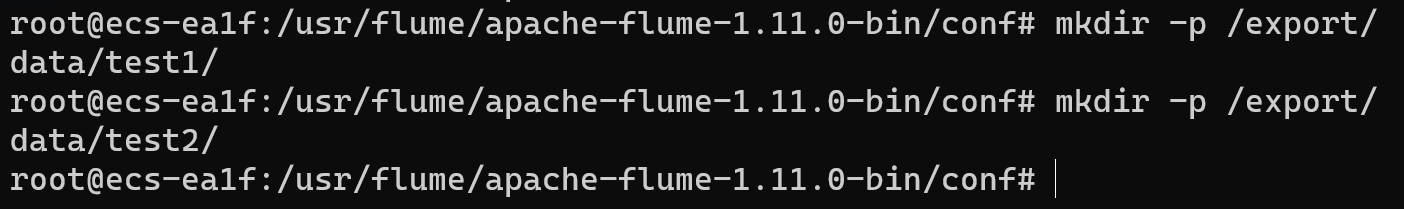
\includegraphics[width=\textwidth]{figure/新建文件夹.png}
  \caption{新建文件夹}
  \label{fig:my_label}
\end{figure}
\begin{figure}[H]
  \centering
  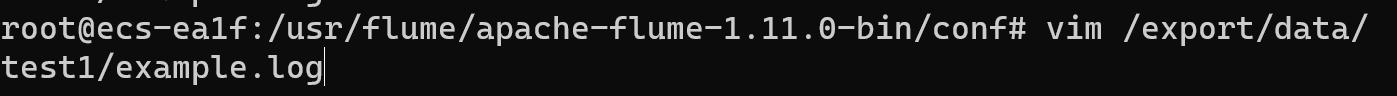
\includegraphics[width=\textwidth]{figure/新建.log.png}
  \caption{新建.log}
  \label{fig:my_label}
\end{figure}

\subsection{启动flume}
\begin{figure}[H]
  \centering
  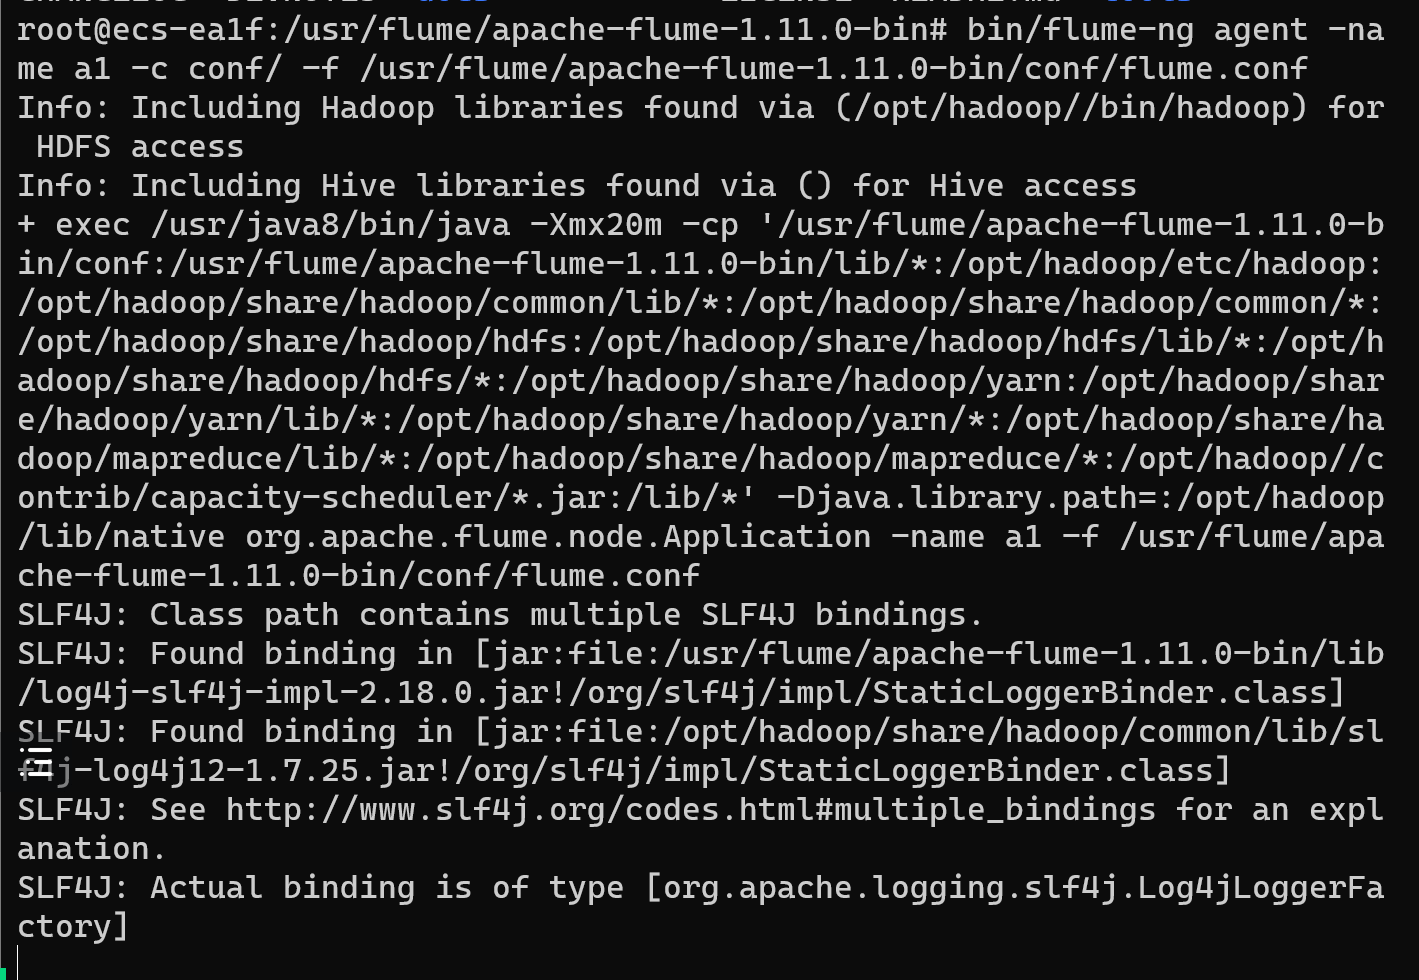
\includegraphics[width=\textwidth]{figure/启动flume.png}
  \caption{启动flume}
  \label{fig:my_label}
\end{figure}
\begin{figure}[H]
  \centering
  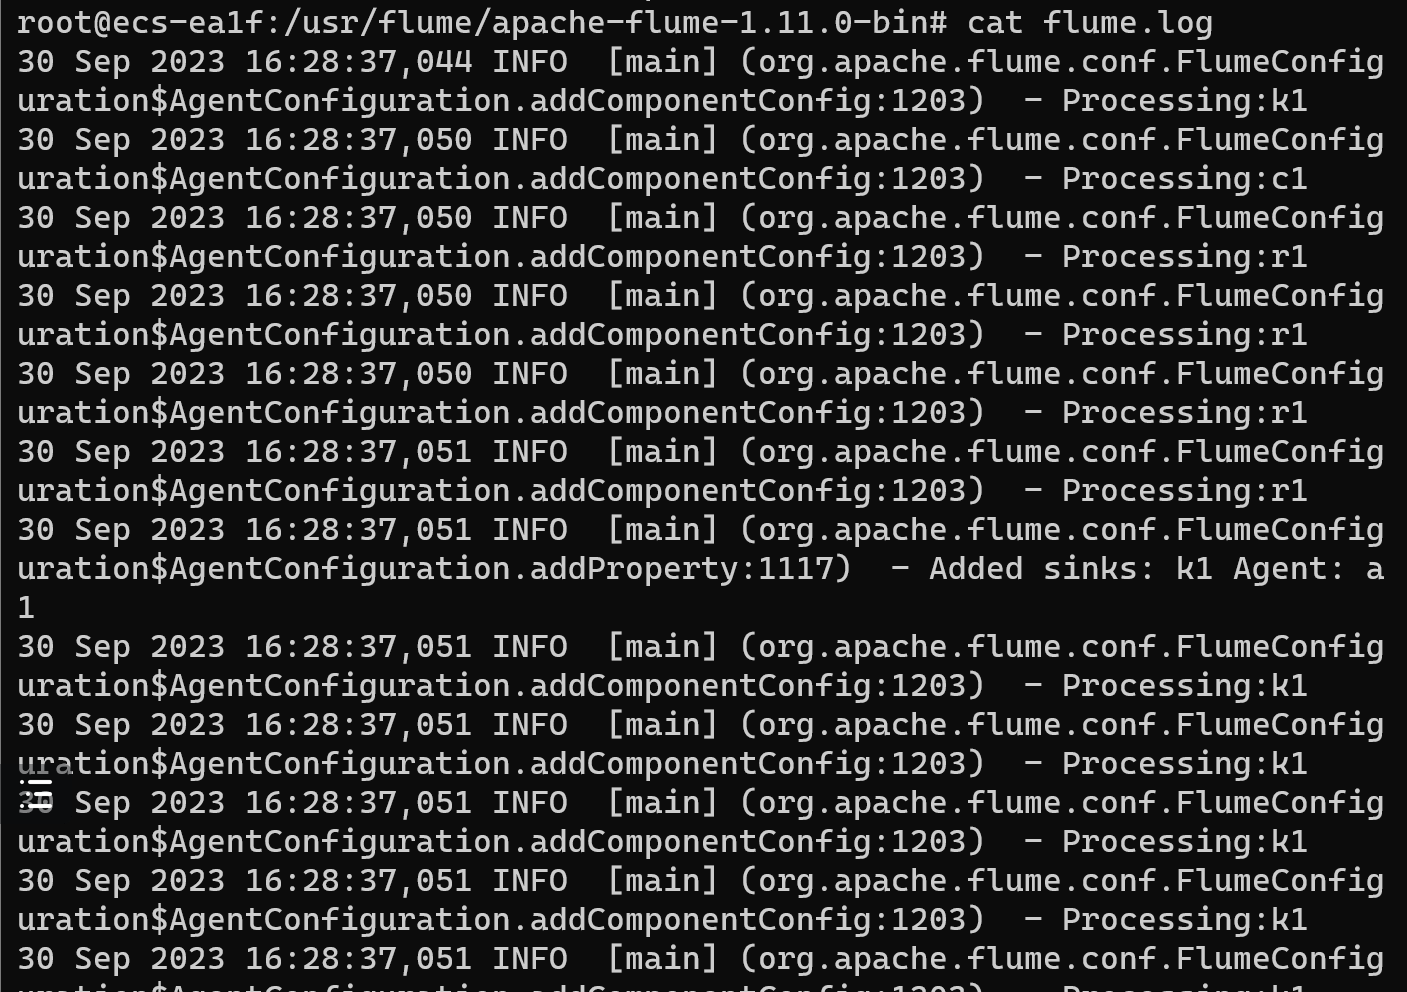
\includegraphics[width=\textwidth]{figure/启动成功.png}
  \caption{启动成功}
  \label{fig:my_label}
\end{figure}

\subsection{写入example.log文件}
向example.log文件中写入数据
\begin{figure}[H]
  \centering
  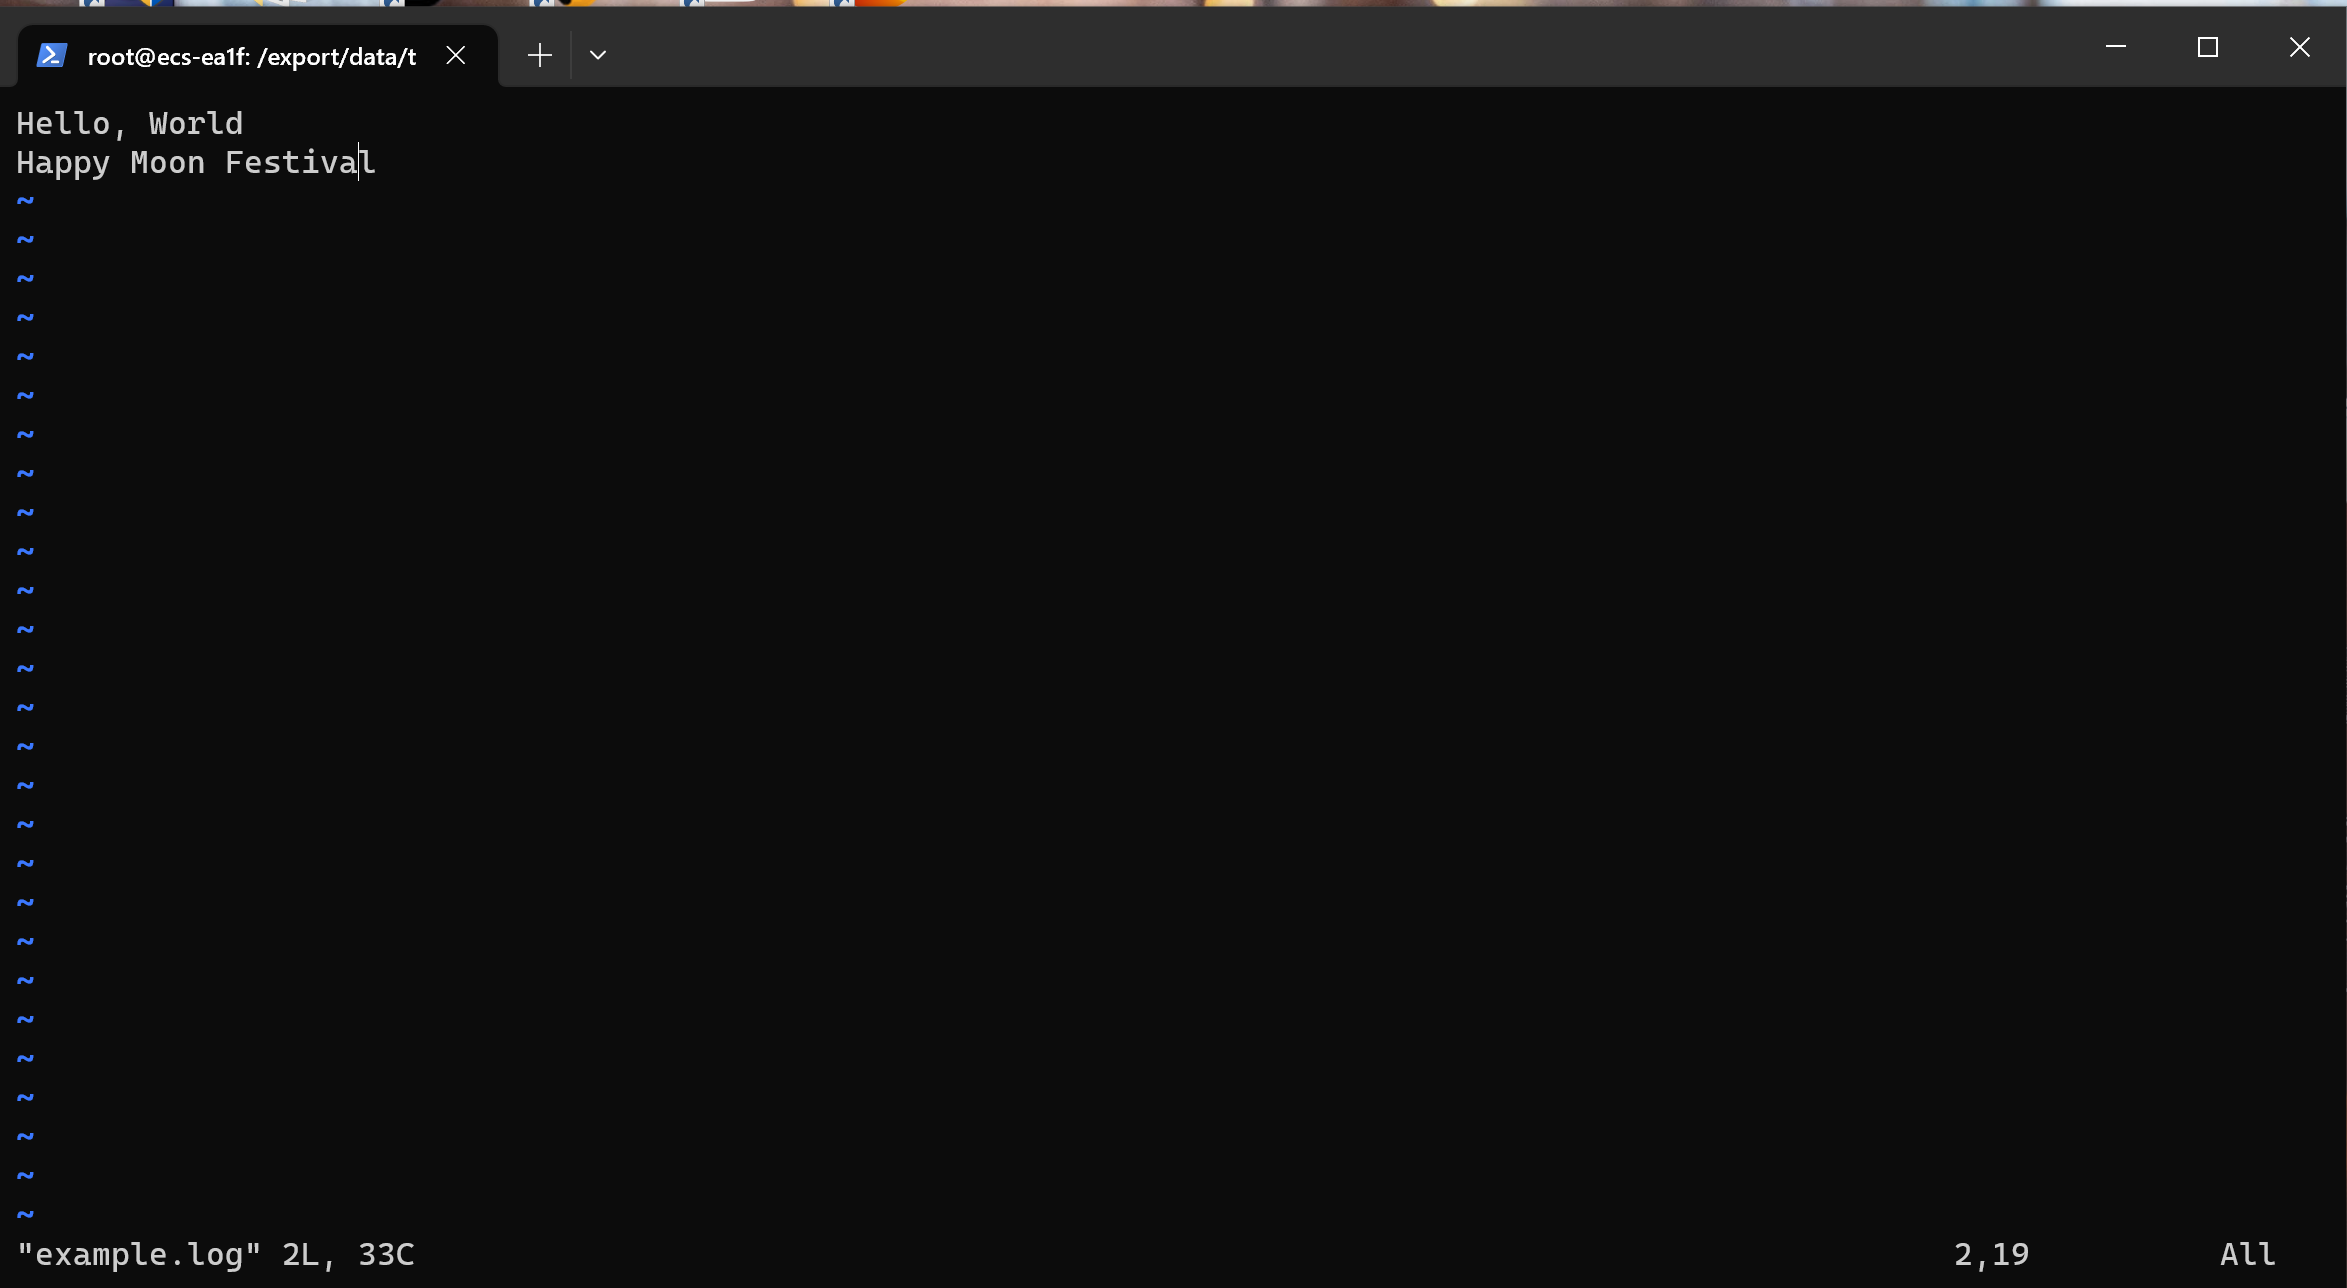
\includegraphics[width=\textwidth]{figure/image.png}
  \caption{50070}
  \label{fig:my_label}
\end{figure}

\subsection{查看50070端口}
通过服务器的公网IP访问50070端口,可以看到.tmp文件
\begin{figure}[H]
  \centering
  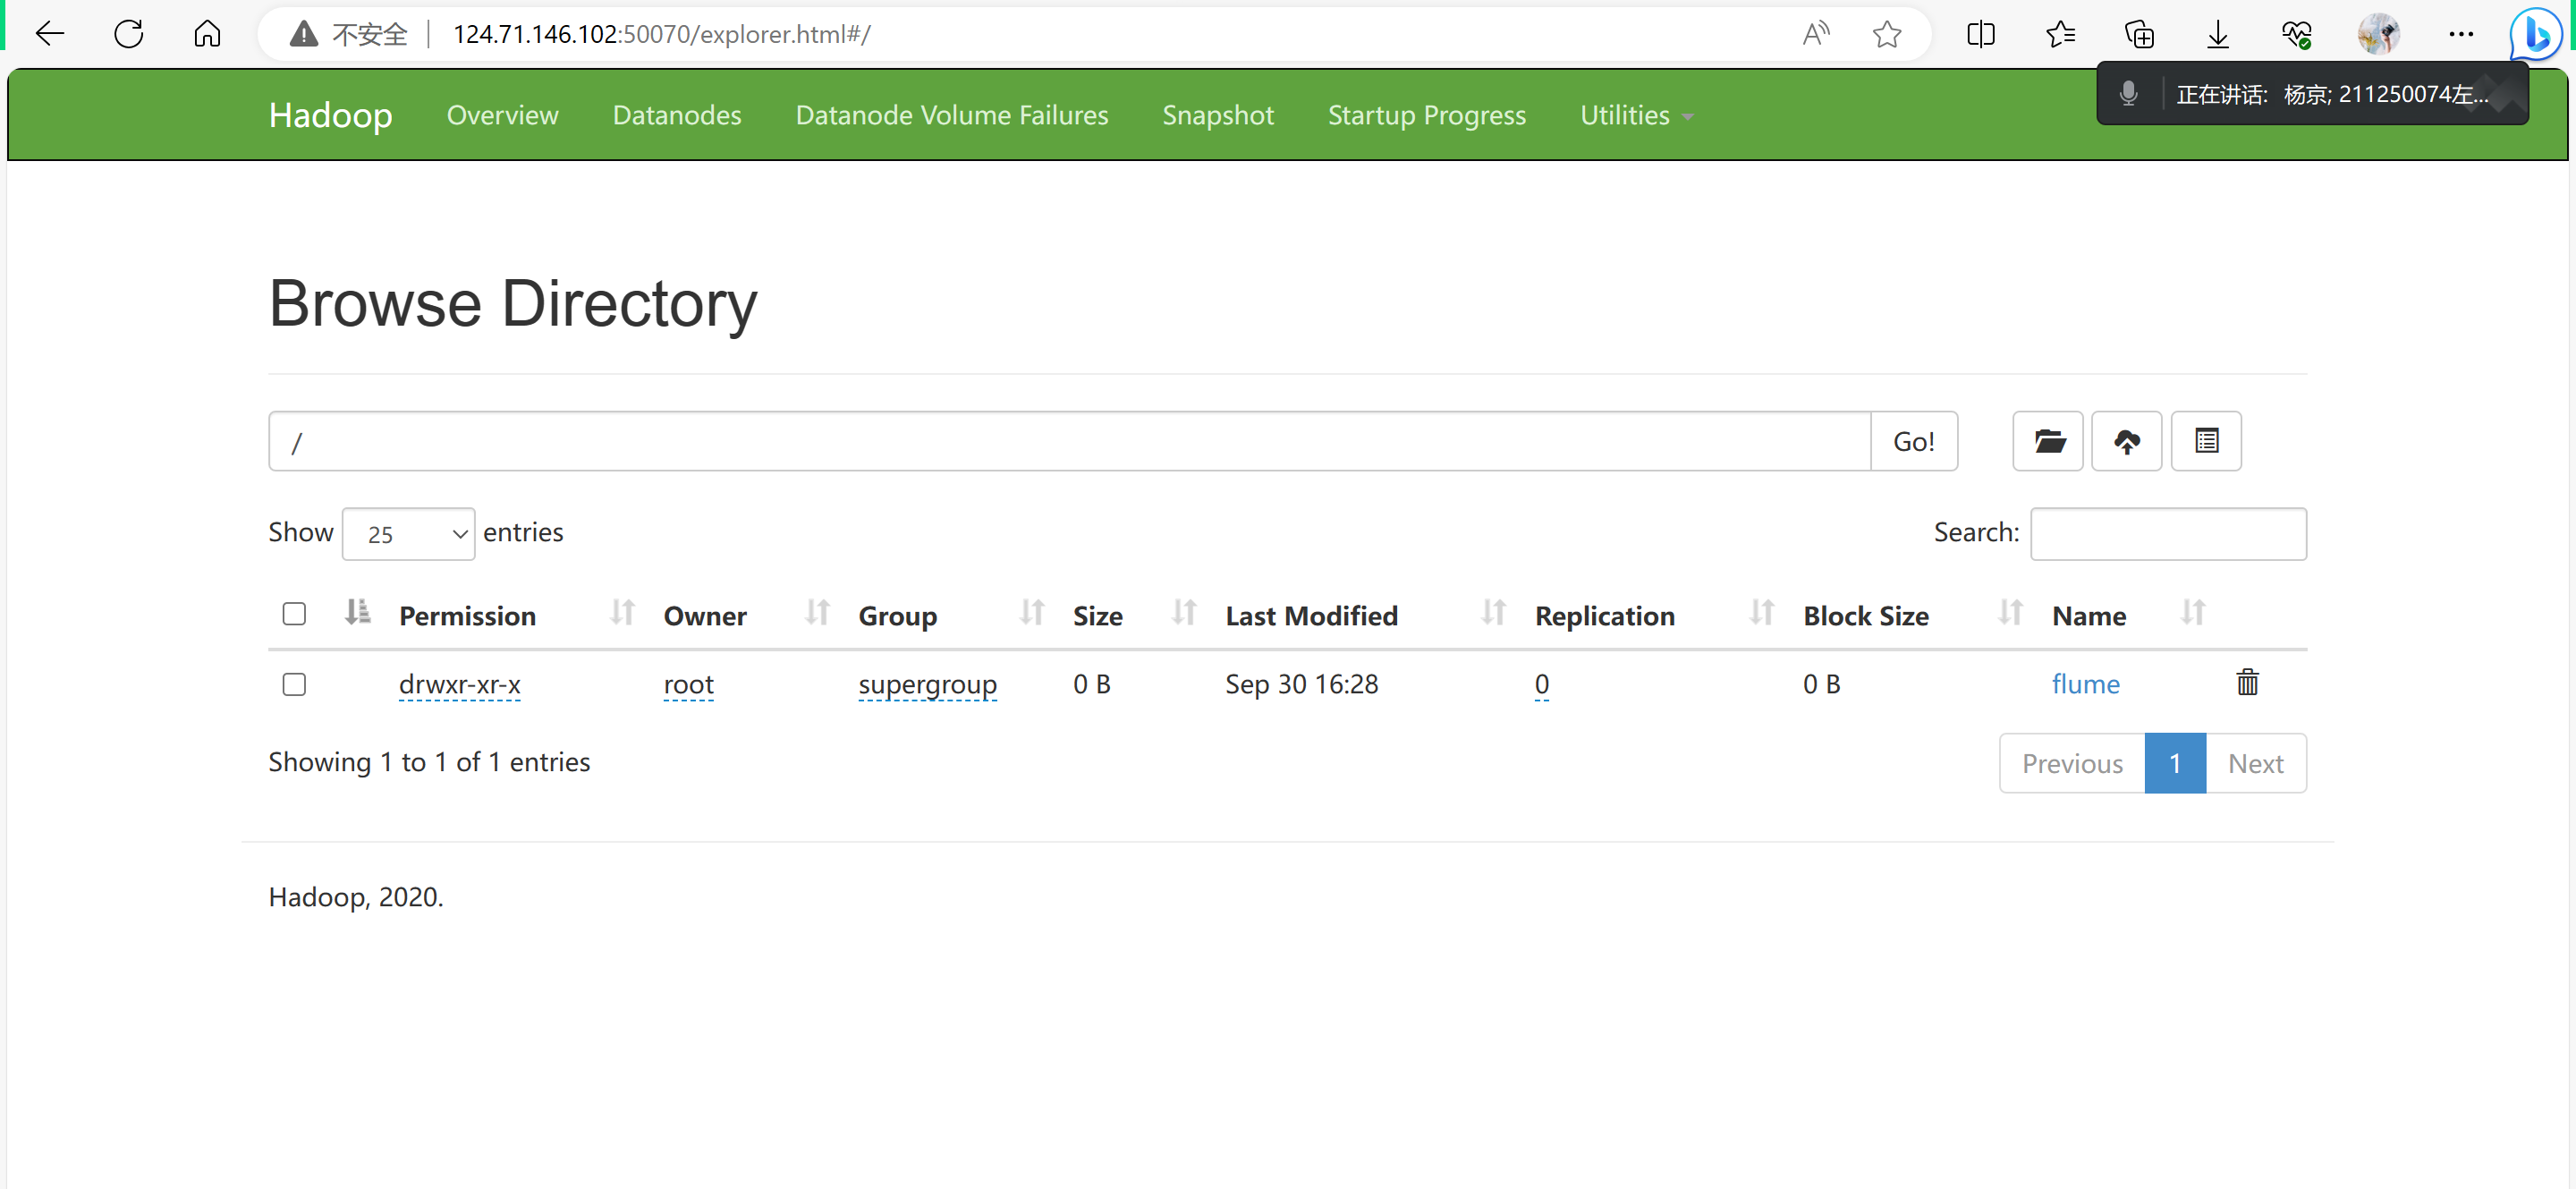
\includegraphics[width=\textwidth]{figure/50070.png}
  \caption{50070}
  \label{fig:my_label}
\end{figure}
\begin{figure}[H]
  \centering
  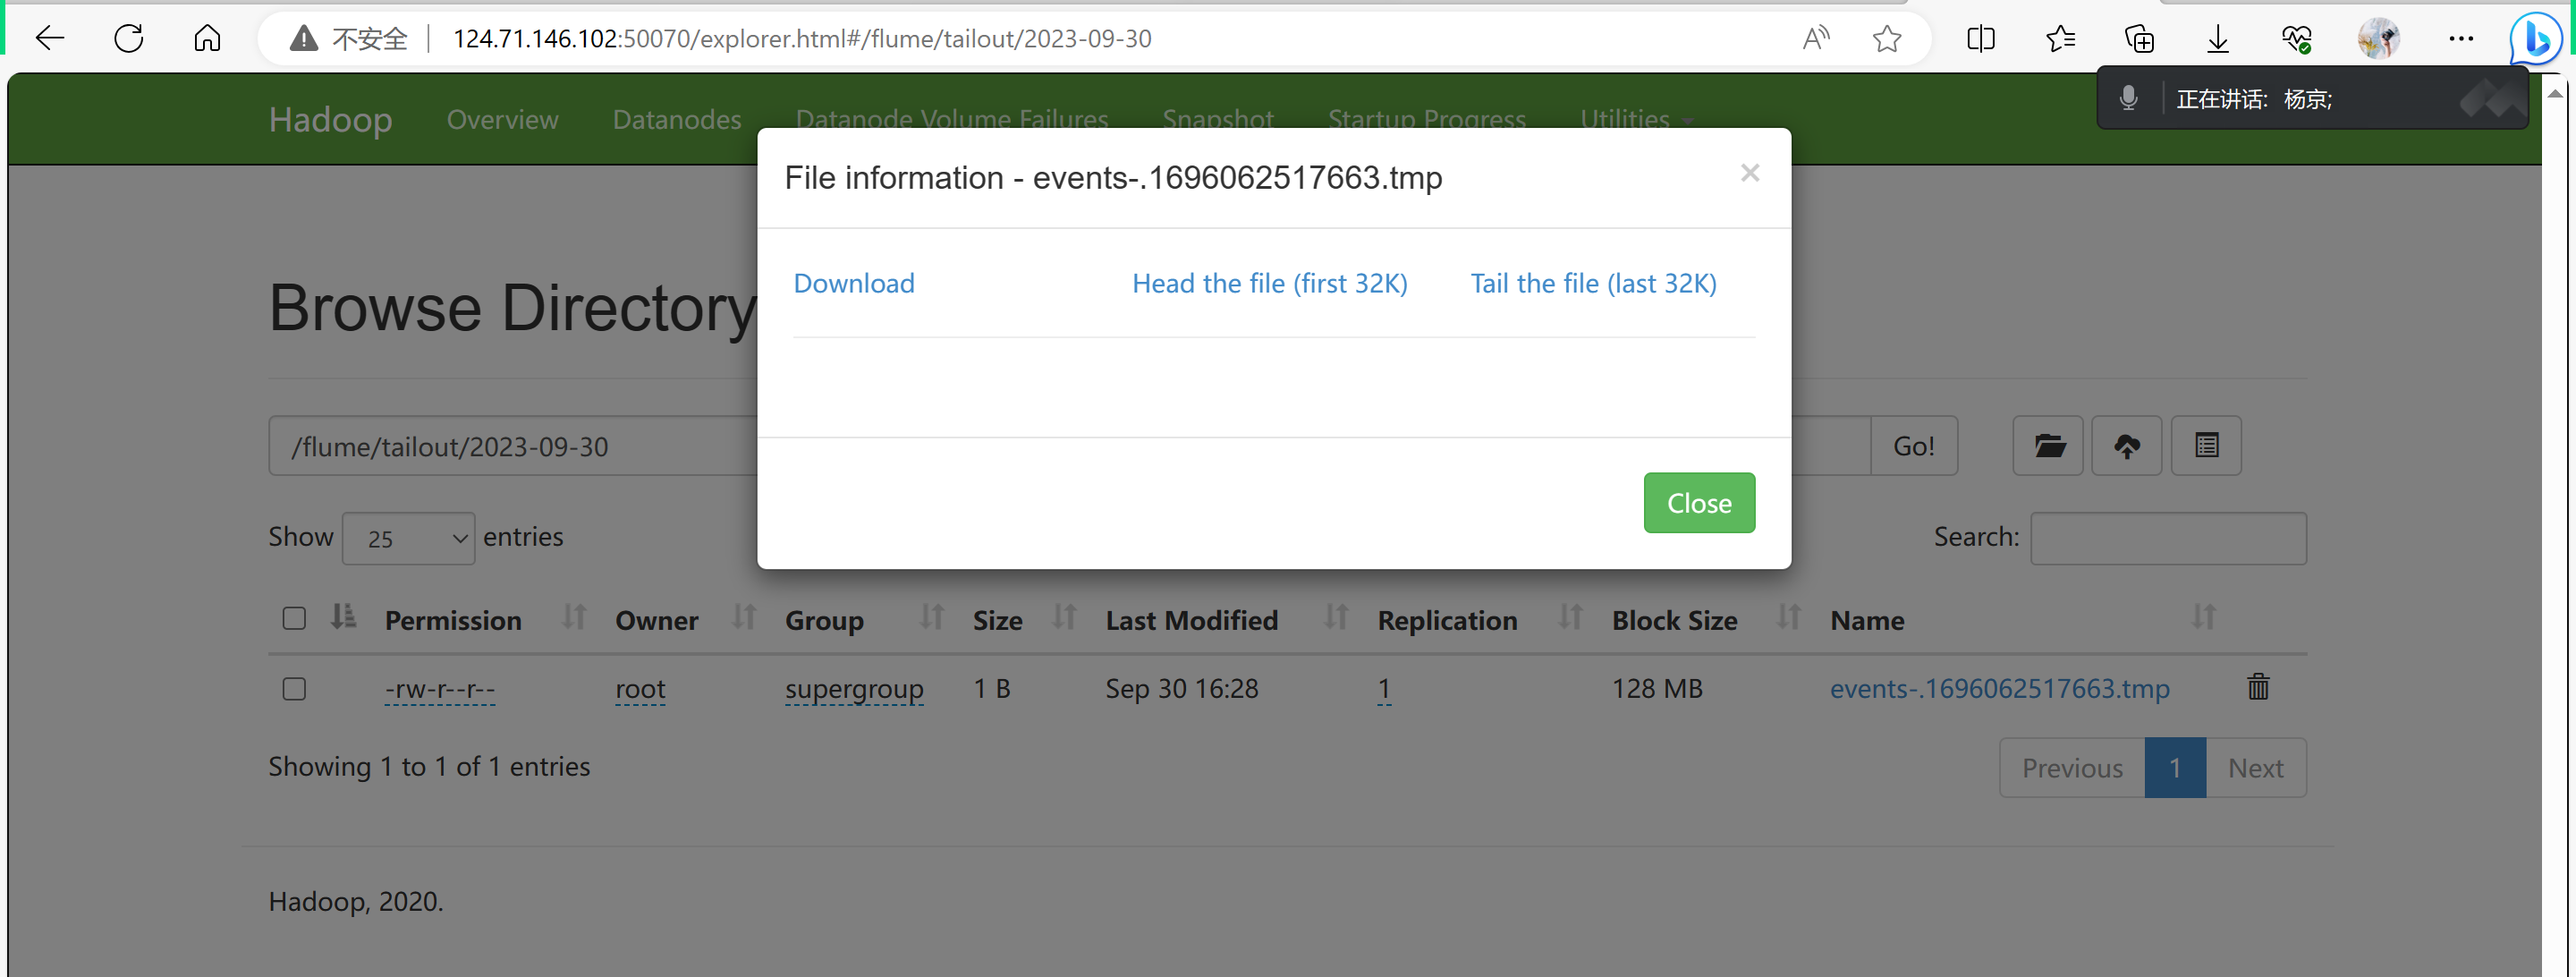
\includegraphics[width=\textwidth]{figure/文件.png}
  \caption{50070}
  \label{fig:my_label}
\end{figure}

\subsection{查看.tmp文件}
通过命令行查看.tmp文件,成功看到example.log中我们写入的信息
\begin{figure}[H]
  \centering
  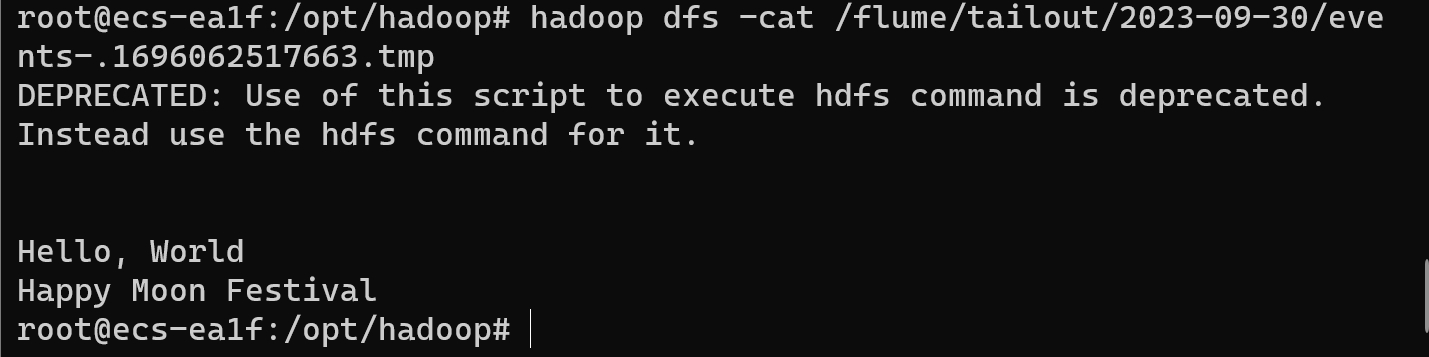
\includegraphics[width=\textwidth]{figure/成功查看到.png}
  \caption{成功查看到}
  \label{fig:my_label}
\end{figure}

成功实现了使用Flume收集日志,实验成功

\section{实验中遇到的困难}
\subsection{任务一}
任务一较为简单,并且再kafka的官网提供了较为详近的手册,在实验的过程中比较顺利,未遇到较大的困难。
\subsection{任务四}
任务四涉及到hadoop和flume,遇到的最大困难是flume中的配置文件如何使用。一开始使用了几个网络上的配置文件,均无法成功实验。后来通过去学习了解配置文件中的每一行的意思,找到了合适的配置文件。\\
另外,在50070端口的图形界面中查看event文件会有延迟,让我一度怀疑自己没有实验成功。后来通过命令行打开.tmp文件,成功查看到了信息。